
\section{Additional Results for Preliminary Study}\label{app:pre}

In this section, we provide the full results of the preliminary study in Section~\ref{sec:pre} 
on CIFAR10, CIFAR100 and Tiny~ImageNet, to illustrate the distinct behaviors of the memorization effect between traditional ERMs and adversarial training. In both ERM and adversarial training, we train the models under ResNet18 and WideResNet28-10 (WRN28) architectures. In the experiments, we train the models for 200 epochs with learning rate 0.1, momentum 0.9, weight decay 5e-4, and decay the learning rate by 0.1 at the epoch 150 and 200. For adversarial training, we conduct experiments using PGD adversarial training~\cite{madry2017towards} by default to defense against $l_\infty$-8/255 adversarial attack, with the exception on Tiny~ImageNet, which is against $l_\infty$-4/255 attack. For robustness evaluation, we conduct a 20-step PGD attack.


\subsection{Additional Results for Preliminary Study - Section~\ref{sec:pre1}}\label{app:pre1}

In this subsection, we provide more experimental results to validate the statement 
in Section~\ref{sec:pre1}, where we state that fitting atypical samples in adversarial training can only improve the clean accuracy of test atypical samples, but hardly help their adversarial robustness. We provide full empirical results to show that: \textbf{(i)} In traditional ERM, fitting atypical samples improves the clean accuracy of test atypical samples. \textbf{(ii)} In adversarial training, fitting (adversarial) atypical samples improves the clean accuracy of test atypical samples but can hardly improve the adversarial robustness of them. The experimental setting follows Section~\ref{sec:pre1}, where we apply traditional ERM and adversarial training on original CIFAR10, CIFAR100, Tiny~ImageNet datasets. We evaluate the model's clean accuracy and adversarial accuracy on training atypical set $\mathcal{D}_\text{atyp}=\{x_i \in \mathcal{D}: \text{mem}(x_i)> 0.15\}$ and its corresponding test atypical set $\mathcal{D}_\text{atyp}' = \{x'_j \in \mathcal{D}': \text{infl}(x_i,x'_j)> 0.15, \text{for } \forall x_i\in \mathcal{D}_\text{atyp}\}$.


\textbf{(i) Additional Results for Preliminary Study - Section~\ref{sec:pre1} In Traditional ERM}

Fig.~\ref{fig:app_1_11}, Fig.~\ref{fig:app_1_12} and Fig.~\ref{fig:app_1_13} report the performance (clean accuracy) of traditional ERM, which is evaluated on atypical sets under ResNet18 (left) and WRN28 (right) on CIFAR100, CIFAR10 and Tiny~ImageNet. From the figures, we can obverse that fitting atypical samples during training can effectively help the models to achieve good clean accuracy on test atypical samples in all datasets. Note that here we only report clean accuracy as they are not robust against adversarial attacks.

\begin{figure}[h]
\centering
\hspace*{-1cm}
\subfloat[ResNet18.]{
\begin{minipage}[c]{0.3\textwidth}
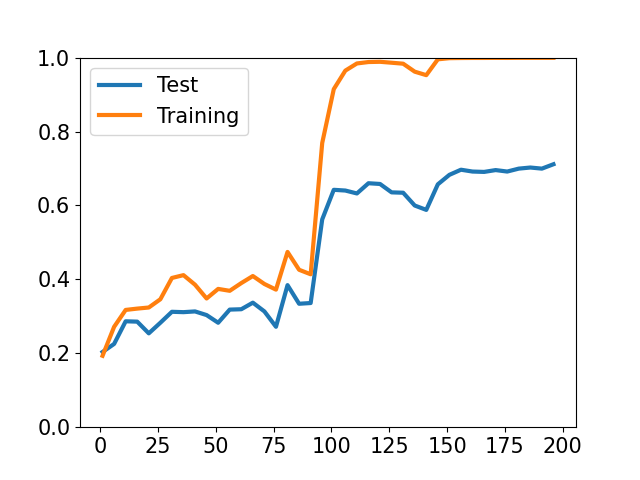
\includegraphics[width = 1.0\textwidth]{figures/pre1_clean_cifar100_ResNet18.png}
\end{minipage}
}
\hspace*{0.4cm}
\subfloat[ WRN28.]{
\begin{minipage}[c]{0.3\textwidth}
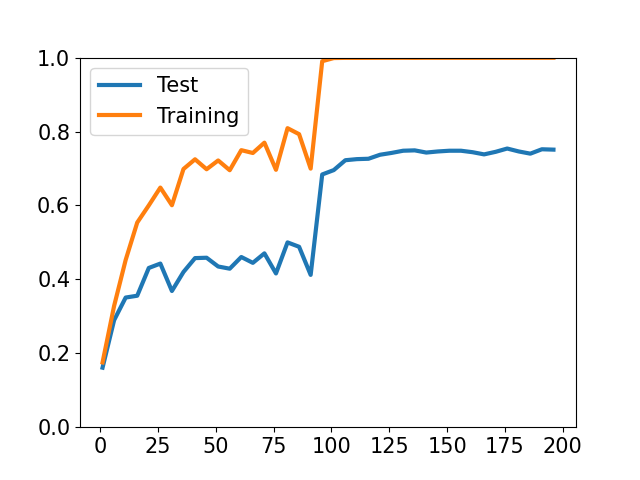
\includegraphics[width = 1.0\textwidth]{figures/pre1_clean_cifar100_WRN28.png}%
\end{minipage}
}
\caption{Clean Accuracy on \textbf{Atypical} Set of CIFAR100}
\label{fig:app_1_11}
\vspace{-0.5cm}
\end{figure}

\begin{figure}[h]
\centering
\hspace*{-1cm}
\subfloat[ ResNet18.]{
\begin{minipage}[c]{0.3\textwidth}
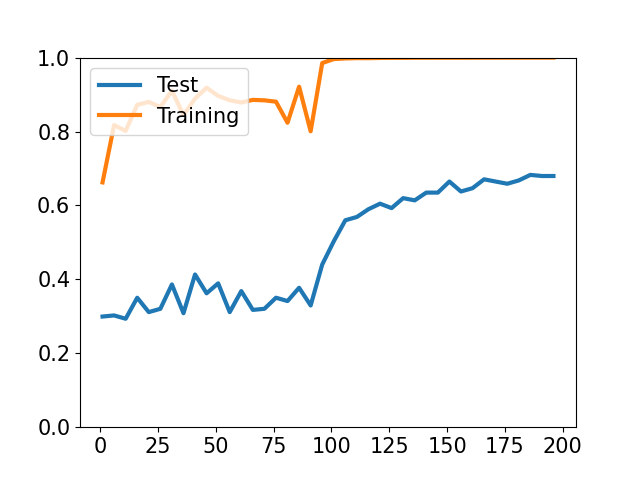
\includegraphics[width = 1.0\textwidth]{figures/pre1_clean_cifar10_ResNet18.png}
\end{minipage}
}
\hspace*{0.4cm}
\subfloat[WRN28.]{
\begin{minipage}[c]{0.3\textwidth}
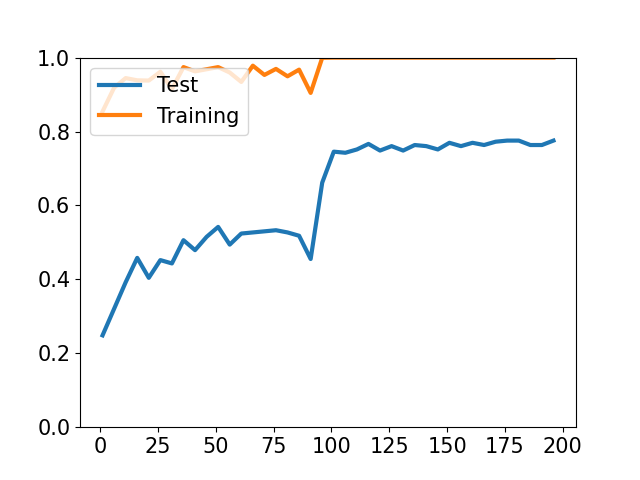
\includegraphics[width = 1.0\textwidth]{figures/pre1_clean_cifar10_WRN28.png}%
\end{minipage}
}
\caption{Clean Accuracy on \textbf{Atypical} Set of CIFAR10}
\label{fig:app_1_12}
\vspace{-0.5cm}
\end{figure}

\begin{figure}[h!]
\centering
\hspace*{-1cm}
\subfloat[ResNet32.]{
\begin{minipage}[c]{0.3\textwidth}
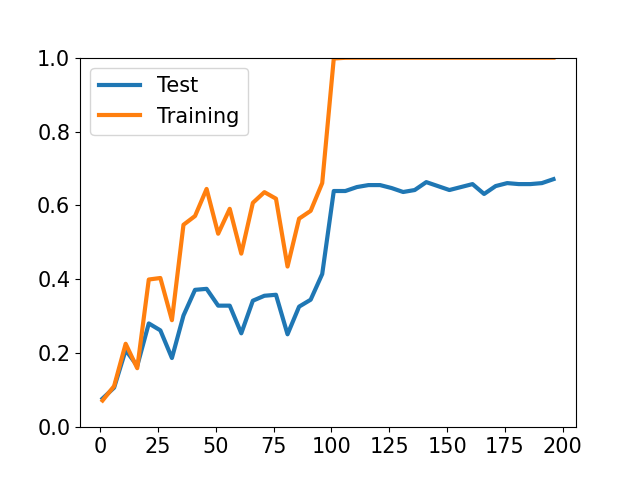
\includegraphics[width = 1.0\textwidth]{figures/pre1_clean_imagenet_ResNet18.png}
\end{minipage}
}
\hspace*{0.4cm}
\subfloat[WRN28.]{
\begin{minipage}[c]{0.3\textwidth}
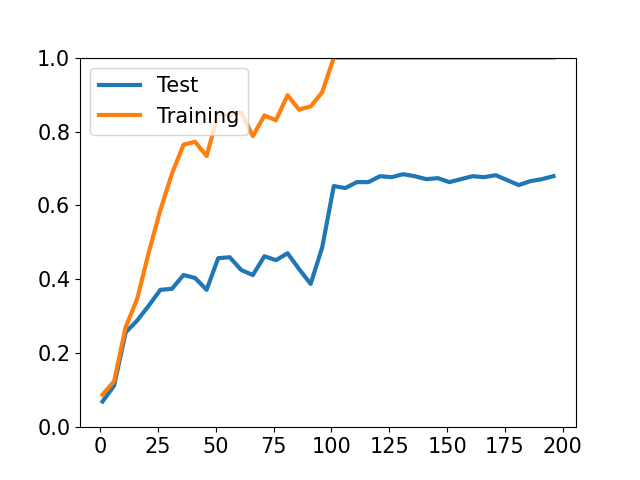
\includegraphics[width = 1.0\textwidth]{figures/pre1_clean_imagenet_WRN28.png}%
\end{minipage}
}
\caption{Clean Accuracy on \textbf{Atypical} Set of Tiny~ImageNet}
\label{fig:app_1_13}
\end{figure}

%%%%%%%%%%%%%%%%%%%%%%%%%%%%%%%%%%%%%%%%%%%%%%%%%%%%%%%%%%%%%%%%%%%%%%%%%%%%%%%%%%%%%%%%%%%%%%%%%%%%%%%%%%%%%%%%%%%%%%%%%%%%%%%%%%%%%%%%%%%%%%%%%%%%%%%%%%%%%%%%%%%%%%%%%%%%%%%%%%%%%%%%%%%%%%%%%%%%%%%%%%%%%%%%%%%%%%%%%%%%%%%%%%%%%%%%%%%%%%%%%%%%%%%%%%%%%%%%%%%%%%%%5

\newpage
\textbf{(ii) Additional Results for Preliminary Study - Section~\ref{sec:pre1} In Adversarial Training}

Fig.~\ref{fig:app_1_21}, Fig.~\ref{fig:app_1_22} and Fig.~\ref{fig:app_1_23} report the performance of adversarially trained models. We evaluate the clean accuracy and adversarial accuracy on the training atypical set $\mathcal{D}_\text{atyp}$ and test atypical set $\mathcal{D}'_\text{atyp}$. From the results, we can observe that although fitting atypical samples can help the model to have modest clean accuracy on test atypical samples, the adversarial robustness of them is constantly low and can hardly be improved during the whole training process.


\begin{figure}[h]
\centering
\hspace*{-1cm}
\subfloat[Clean (left) \& Adv Acc. (right) under ResNet18.]{
\begin{minipage}[h]{0.55\textwidth}
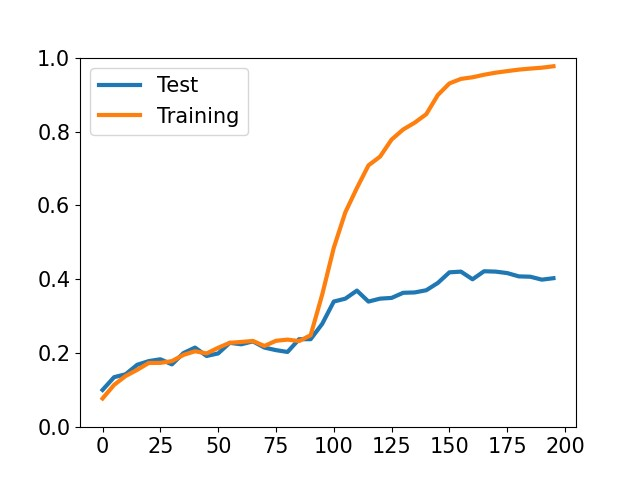
\includegraphics[width = 0.5\textwidth]{figures/clean_rare_cifar.jpg}%
\hfill
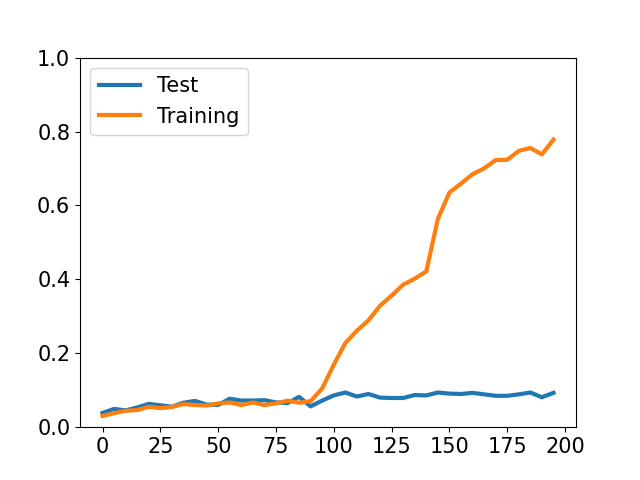
\includegraphics[width = 0.5\textwidth]{figures/adv_rare_cifar100.png}
\end{minipage}
}
\hspace*{-0.4cm}
\subfloat[Clean (left) \& Adv Acc. (right) under WRN28.]{
\begin{minipage}[c]{0.55\textwidth}
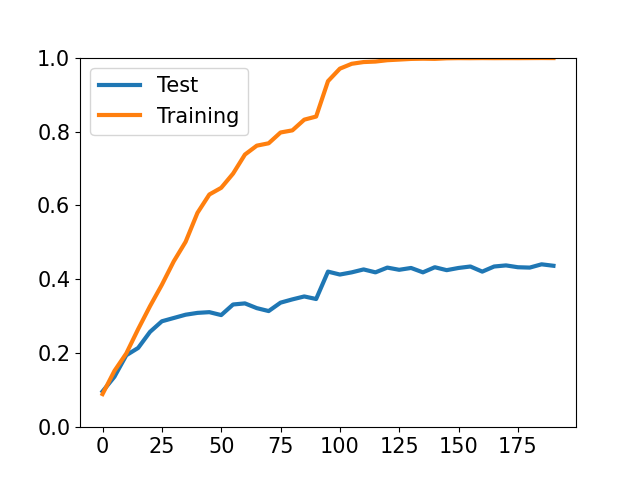
\includegraphics[width = 0.5\textwidth]{figures/wrn_clean_rare_cifar100.png}%
\hfill
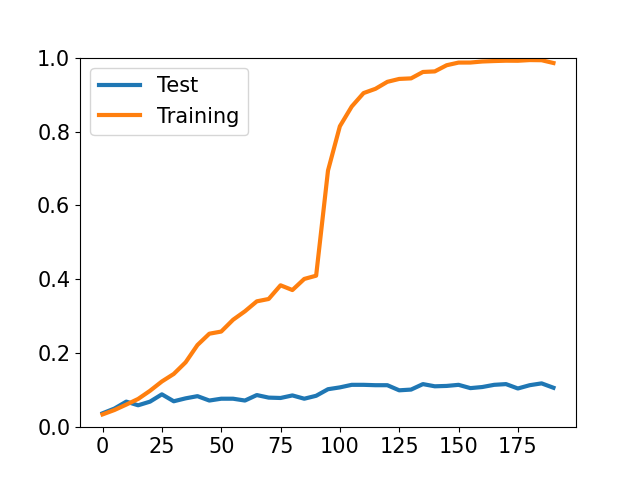
\includegraphics[width = 0.5\textwidth]{figures/wrn_adv_rare_cifar100.png}
\end{minipage}
}
\caption{Clean Accuracy and Adversarial Accuracy on \textbf{Atypical} Set of CIFAR100}
\label{fig:app_1_21}
\vspace{-0.5cm}
\end{figure}

\begin{figure}[h]
\centering
\hspace*{-1cm}
\subfloat[Clean (left) \& Adv Acc. (right) under ResNet18.]{
\begin{minipage}[h]{0.55\textwidth}
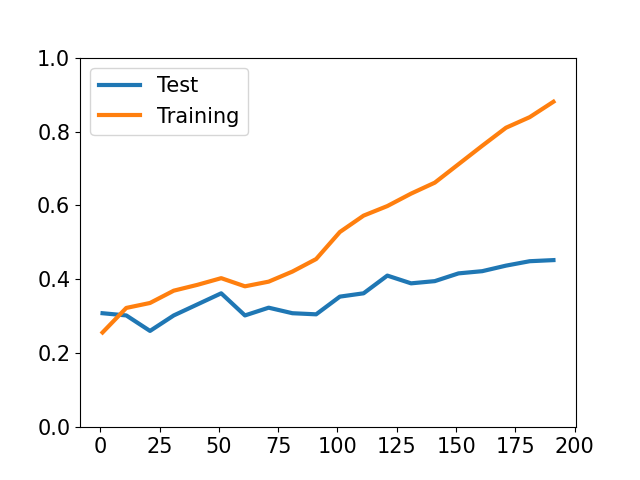
\includegraphics[width = 0.5\textwidth]{figures/pre1_cifar10_adv1_resnet18.png}%
\hfill
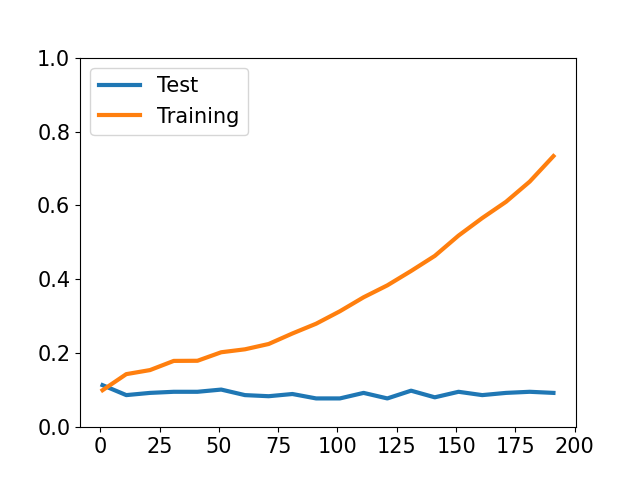
\includegraphics[width = 0.5\textwidth]{figures/pre1_cifar10_adv2_resnet18.png}
\end{minipage}
}
\hspace*{-0.4cm}
\subfloat[Clean (left) \& Adv Acc. (right) under WRN28.]{
\begin{minipage}[c]{0.55\textwidth}
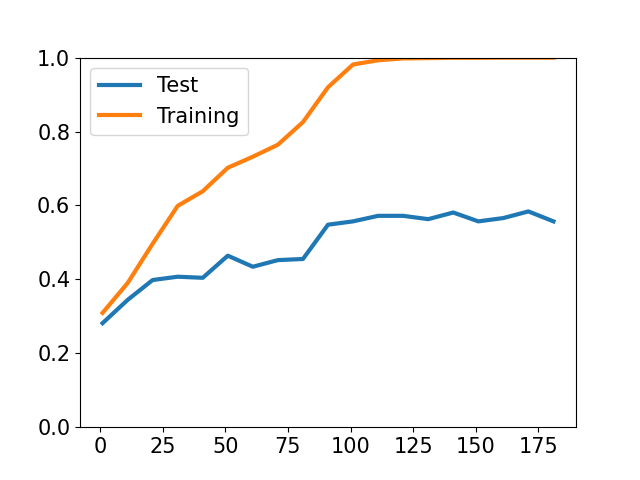
\includegraphics[width = 0.5\textwidth]{figures/pre1_cifar10_adv1_wrn28.png}%
\hfill
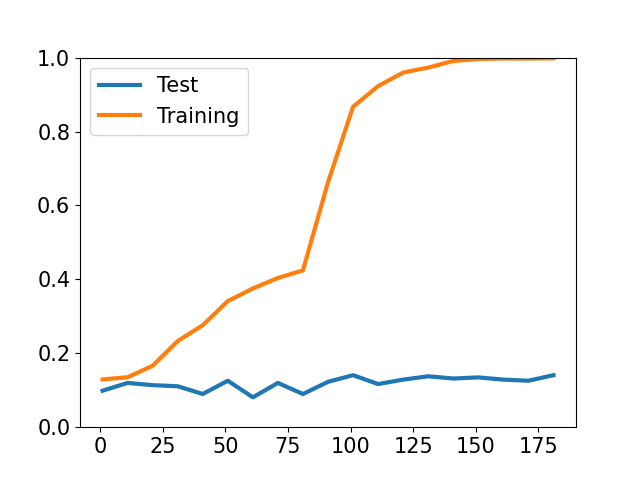
\includegraphics[width = 0.5\textwidth]{figures/pre1_cifar10_adv2_wrn28.png}
\end{minipage}
}
\caption{Clean Accuracy and Adversarial Accuracy on \textbf{Atypical} Set of CIFAR10}
\label{fig:app_1_22}
\vspace{-0.5cm}
\end{figure}

\begin{figure}[h!]
\centering
\hspace*{-1cm}
\subfloat[Clean (left) \& Adv Acc. (right) under ResNet32.]{
\begin{minipage}[h]{0.55\textwidth}
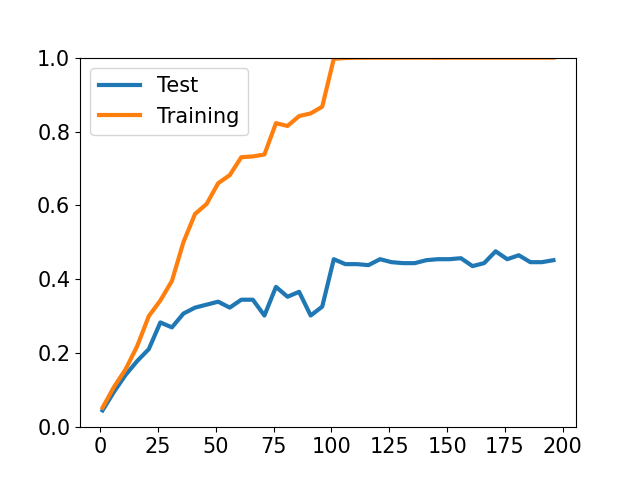
\includegraphics[width = 0.5\textwidth]{figures/pre1_imagenet_adv1_resnet18.png}%
\hfill
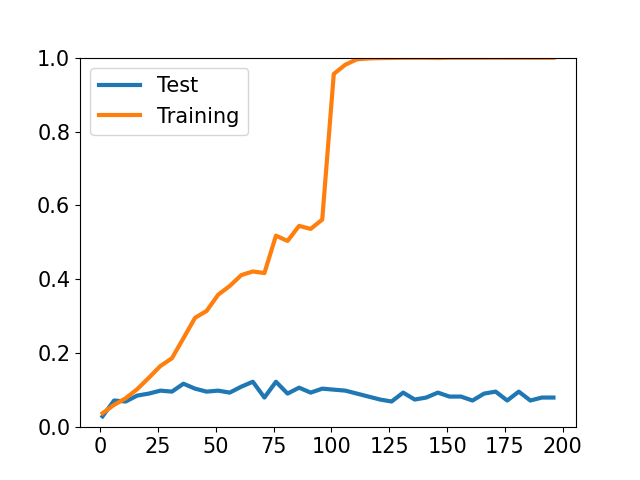
\includegraphics[width = 0.5\textwidth]{figures/pre1_imagenet_adv2_resnet18.png}
\end{minipage}
}
\hspace*{-0.4cm}
\subfloat[Clean (left) \& Adv Acc. (right) under WRN28.]{
\begin{minipage}[c]{0.55\textwidth}
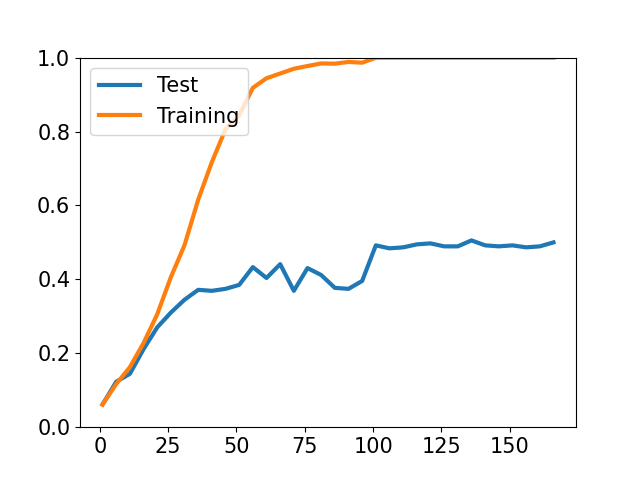
\includegraphics[width = 0.5\textwidth]{figures/pre1_imagenet_adv1_wrn28.png}%
\hfill
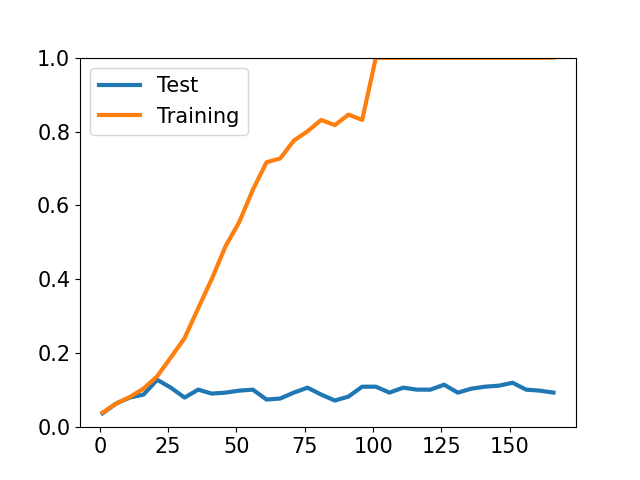
\includegraphics[width = 0.5\textwidth]{figures/pre1_imagenet_adv2_wrn28.png}
\end{minipage}
}
\caption{Clean Accuracy and Adversarial Accuracy on \textbf{Atypical} Set of Tiny~ImageNet}
\label{fig:app_1_23}
\end{figure}
